\documentclass[12pt,twoside,book]{article}
\usepackage{docmute}

\input{../settings}

\begin{document}

%%%%%%%%%%%%%%%%%%%%%%%%%%%%%%%%%%%%%%%%%%%%%%%%%%%%%%%%%%%%%%%%%%%%%%%%%%%%%%%
\section{Direct collider search of WIMPs}
\setcounter{equation}{0}
%%%%%%%%%%%%%%%%%%%%%%%%%%%%%%%%%%%%%%%%%%%%%%%%%%%%%%%%%%%%%%%%%%%%%%%%%%%%%%%

\vskip 0.1in

In this section, we review the production of $\mathrm{TeV}$-scale WIMPs and search for their signals using the collider experiment.
In particular, we will summarize the current bounds for WIMPs obtained at the large hadron collider (LHC) and future bounds expected at the future planned $100\,\mathrm{TeV}$ colliders such as the hadron option of the future circular collider (FCC-hh) \cite{Benedikt:2651300} and the super proton-proton collider (SPPC) \cite{CEPC-SPPCStudyGroup:2015csa, CEPC-SPPCStudyGroup:2015esa}.
In Sec.~\ref{sec:wimp_production}, we discuss the dominant production processes of WIMPs at a hadron collider.
In Sec.~\ref{sec:disappearing_track} and \rem{???}, we review \rem{two???} different methods for the signal identification, the disappearing track search and mono-jet search \rem{???}, and summarize the current and future bounds.


%%%%%%%%%%%%%%%%%%%%%%%%%%%%%%%%%%%%%%%%%%%%%%%%%%%%%%%%%%%%%%%%%%%%%%%%%%%%%%%
\subsection{WIMP production}
\label{sec:wimp_production}
%%%%%%%%%%%%%%%%%%%%%%%%%%%%%%%%%%%%%%%%%%%%%%%%%%%%%%%%%%%%%%%%%%%%%%%%%%%%%%%

There are two relevant processes both of which significantly contribute to the WIMP production cross section.
The pair production via electroweak interaction is a universal process that can be considered for any WIMP considered in this thesis.
The decay of colored particles may also be efficient particularly for the MSSM.
In this subsection, we will review these two in order.


\subsubsection*{Pair production via electroweak interaction}

\begin{figure}[b]
  \centering
  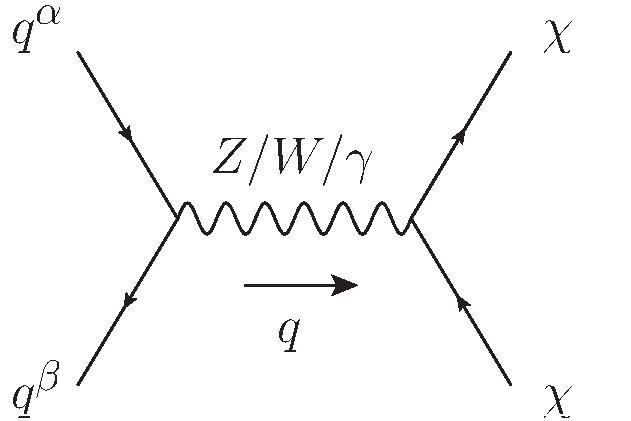
\includegraphics[width=0.4\hsize]{WIMP_production.pdf}
  \caption{WIMP pair production process at the hadron collider.}
  \label{fig:wimp_production}
\end{figure}

Since all the WIMPs considered here possess non-zero $SU(2)_L$ and $U(1)_Y$ charges, they can be directly produced via electroweak interaction at the hadron collider as shown in Fig.~\ref{fig:wimp_production}.
In the figure, $q^a$ and $q^b$ denote the partons of the incident protons relevant for the process, while $\chi$ denotes the WIMP and $q$ is the momentum transfer.
Assuming the WIMP to be a $SU(2)_L$ $n$-plet with $U(1)_Y$ charge $Y$ and the mass $m_\chi$, this process is well described by the effective lagrangian
\footnote{
  In this subsection, we neglect the small mass difference among different components in the multiplet $\chi$ described in \ref{sec:disappearing_track}.
  This approximation is valid since the mass difference is by far smaller than $m_\chi$ and has only a tiny effect on the production process.
}
\begin{align}
  \mathcal{L} &= \mathcal{L}_{\mathrm{SM}} + (D^\mu \chi)^\dagger (D_\mu \chi) - m_\chi^2 \chi^\dagger \chi &
  &\text{(complex scalar)}, \label{eq:lag_scalar}\\
  \mathcal{L} &= \mathcal{L}_{\mathrm{SM}} + \bar{\chi} (i \Slash{D} - m_\chi) \chi &
  &\text{(Dirac fermion)}, \label{eq:lag_fermion}
\end{align}
with $\mathcal{L}_{\mathrm{SM}}$ being the SM lagrangian, while the covariant derivative is given by
\begin{align}
  D_\mu \equiv \partial_\mu - i g_2 \Slash{W}^a T_n^a - i g_1 Y \Slash{B},
\end{align}
where $T_n^a$ ($a=1,2,3$) are $n$-dimensional representation matrices of $SU(2)_L$.
Note that when $\chi$ is a real scalar (Majorana fermion) with $Y=0$, the terms with $\chi$ in Eq.~\eqref{eq:lag_scalar} (Eq.~\eqref{eq:lag_fermion}) should be devided by two.

For the calculation, we neglect the effect of the electroweak symmetry breaking, which is valid because we are interested in the high-energy collision with the parton-level center-of-mass (CM) energy $\sqrt{s'} \equiv \sqrt{q^2} \gsim \mathrm{TeV}$.
Then, we consider the process in the CM frame and estimate the parton-level differential cross section as
\rem{Scalar case!!}
\begin{align}
  \left. \frac{d \sigma_{a b}}{d \sqrt{s'} d \Omega} \right|_{\text{CM}}
  = \frac{C}{4 s'} \sqrt{1 - \frac{4 m_\chi^2}{s'}}
  \left[ 1 + \frac{4 m_\chi^2}{s'} + \left( 1 - \frac{4 m_\chi^2}{s'} \right) \cos^2 \theta \right],
\end{align}
where $\theta$ is the angle between the momentum of the initial parton $q_a$ and that of one of the final state WIMPs.
Note that this expression represents an inclusive cross section, \textit{i.e.} the total cross section for the production of any component of the WIMP multiplet $\chi$.
The coefficient $C$ consists of contributions from $U(1)_Y$ and $SU(2)_L$ gauge bosons,
\begin{align}
  C = Y^2 \alpha_1^2 + \frac{3}{2} I(n) \alpha_2^2,
\end{align}
with $I(n)$ being the Dynkin index for the $n$-dimensional representation given by
\begin{align}
  I(n) \equiv \frac{n^3-n}{12}.
\end{align}
Recalling that $\alpha_1 < \alpha_2$ and that we often consider the WIMPs with large $n$ and moderate $Y$, this cross section grows as $n^3$ for larger multiplets.

As is well-known, the initial state of the hadron collider is not the individual partons like quarks and gluons but two protons.
To obtain the cross section for the two protons initial state, we rely on the parton distribution function (PDF), which expresses the fraction of the partons with some given momentum in each accelerated proton.
Let $f_a (x)$ ($0 < x < 1$) be the PDF for a given parton $a$ inside a proton with momentum $p^\mu$.
$f_a (x)$ can be interpreted as a probability distribution to find the parton $a$ with momentum $x p^\mu$, so we have a relationship
\begin{align}
  \sum_a \int_0^1 dx \, x f_a (x) = 1,
\end{align}
associated with the total momentum conservation, and
\begin{align}
  \int_0^1 dx \, \left[ f_d (x) - f_{\bar{d}} (x) \right] &= 1,\\
  \int_0^1 dx \, \left[ f_u (x) - f_{\bar{u}} (x) \right] &= 2,
\end{align}
from the composition of the proton.
Using the PDF, the cross section for the process of interest at the hadron collider is evaluated as
\begin{align}
  \frac{d \sigma}{d \sqrt{s'} d \Omega} =
  \sum_{a,b} \int_0^1 dx_1 dx_2 \, f_a (x_1) f_b (x_2) \delta \left( s' - s x_1 x_2 \right)
  \left. \frac{d \sigma_{a b}}{d \Omega} \right|_{\text{lab}},
\end{align}
where $\sqrt{s}$ is the CM energy of the proton-proton collision.
Note that the cross section in the integrand is a function of $x_1$ and $x_2$, which is obtained by performing the appropriate Lorentz transformation to $\left. d \sigma_{a b} / d \Omega\, \right|_{\text{CM}}$.

\rem{Table of cross sections}

\rem{Histogram of angular dependence}

\rem{Is angular dependence affected by the Lorentz boost?}


\subsubsection*{Decay of colored particles}


%%%%%%%%%%%%%%%%%%%%%%%%%%%%%%%%%%%%%%%%%%%%%%%%%%%%%%%%%%%%%%%%%%%%%%%%%%%%%%%
\subsection{Disappearing track search}
\label{sec:disappearing_track}
%%%%%%%%%%%%%%%%%%%%%%%%%%%%%%%%%%%%%%%%%%%%%%%%%%%%%%%%%%%%%%%%%%%%%%%%%%%%%%%

\rem{Histogram of surviving probability}

\rem{Histogram of beta distribution before / after 10cm cut}

\bibliographystyle{elsarticle-num}
\bibliography{../phd}

\end{document}
